In this chapter we present  \namens,  an open source framework for Systematic Comparative Research on RSP Engine.
It consists in four baselines and two main components: the Test Stand and the Analyser. Firstly, Section \ref{sec:teststand} introduces the Test Stand, which satisfies requirements from R.1 to R.8 and from R.10 to R.12, by executing experiments on an RSP Engine. Section \ref{sec:baselines} describes the Baselines, four RSP Engines that are included in \name as naive terms of comparison, since they fulfil requirements R.13 and R.14. Finally, Section \ref{sec:analyser} presents the Analyser, which addresses requirements R.9 and R.10  allowing the user to visualise, investigate and compare experiment results. %Soundness and completes of the query answering process are assessed post-hoc by comparing the results of an RSP engine with a term of comparison whose results are correct (see Section 5).

\section{Test Stand}\label{sec:teststand}

Aerospace engineering defines an Engine Test Stand as a facility used to develop, study and characterise engines. It allows to test operating regimes and offers measurement of several variables associated with engine process. A Test Stand may uses actuators for attaining a specific engine state, which is a unique combination of the engine properties. The information collected through the sensors depends on the engine manufacturer, which usually provides his own stand or the facilities to test the engine with commercial solutions. The Test Stand executes black box analysis, because usually the engines does not allow easily to interact with its internal mechanisms.

A Test Stand can be described similarly in the SR context. The definition above still holds its relevance with the difference that the tested engines are IO-Systems. An RSP Engine consumes an RDF Stream and  produces a new one, by applying queries under some entailment regime and w.r.t. an ontology which does not change over time. Describeing an RSP Engine means understanding the relation between input stream, the queries registered to it and what we call "operational semantics", which requires to know the RSP Engine internal process. Indeed, black box testing is the only possible one with a Test Stand, even having access to the entire RSP Engine code. Anyhow, \name Test Stand allows the user (the RSP Engine developer) to extend the sensors set add its own ones, according to requirements R.7 and R.10. In this way is possible to develop a specific testing procedure for a given engine.

\subsection{Architecture \& Workflow}\label{sec:arch-workflow}

\begin{figure}[tbh]
\centering
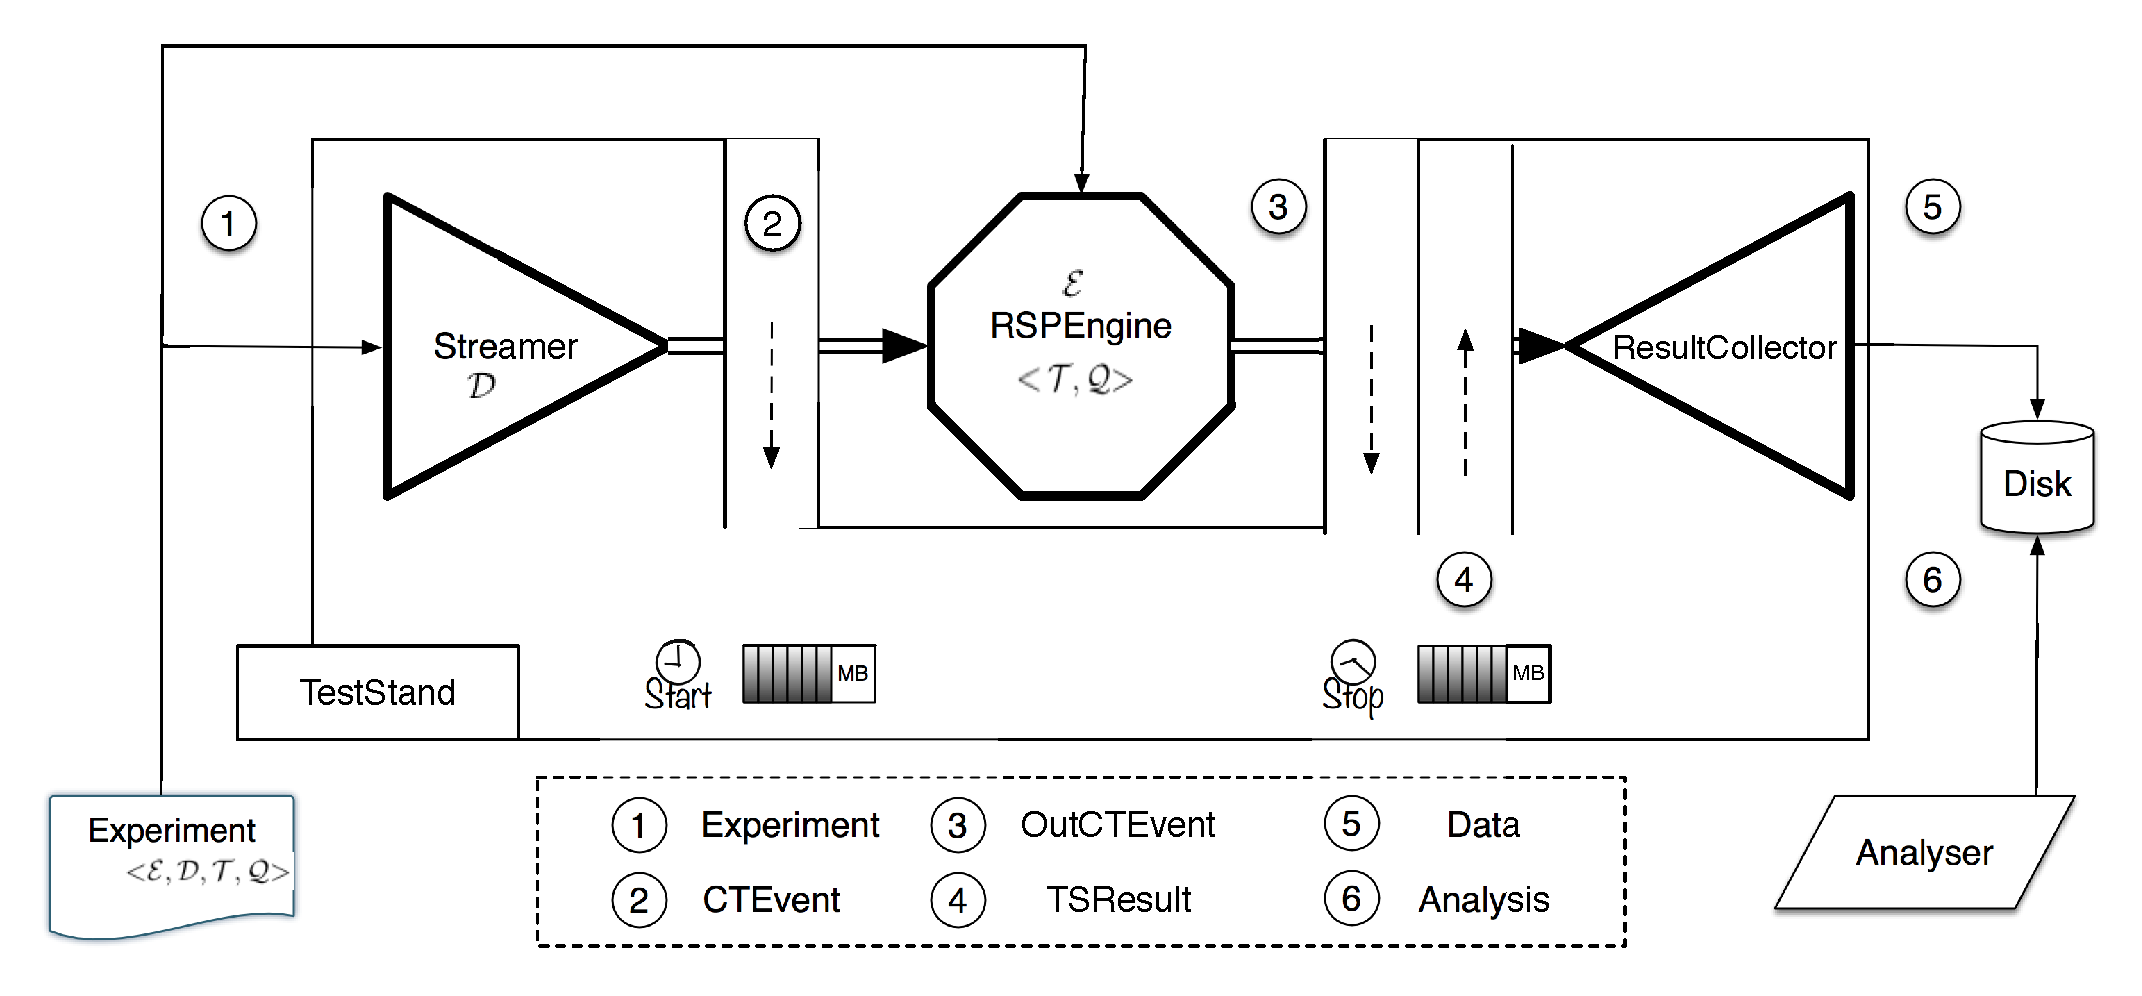
\includegraphics[scale=0.37]{images/schema2}
\caption{\name modules and workflow} 
\label{fig:architecture}
\end{figure}

\noindent An aerospace test stand exploits different modules to simulate the operating regime for the engine in use ( i.e a module for fuel distribution, one for the engine mechanic support or to enable users interaction during the execution ). \name \textsc{Test Stand}  is modular, it consists in stand-alone components that can be replaced with ones with the same interfaces [R.10]. At this moment, three modules compose the \textsc{Test Stand}:
\begin{itemize}
\item the \textsc{Streamer}, a source for the input RDF Stream
\item the RSP Engine we want to test;
\item the \textsc{Result Collector}, a data acquisition system for both the query results and the gathered measurements.
\end{itemize}
Figure \ref{fig:architecture} shows both the architecture of \name TS and its workflow.

We start presenting how the modules are configured: the components above are arranged into a pipeline and communicates exchanging events [R.11].  The execution starts with the \textsc{Streamer}, which hides the data generation logic in order to obtain data independence [R.1]. It pushes an RDF Stream directly to the mounted RSP Engine. It is up to the \textsc{Streamer} to respect [R.5] and not to influence the memory footprint with heavy data loading tasks. 

An interface adapts the event flow to the RSP Engine in use, fulfilling [R.2] (Engine Independence) and hiding the query registration process [R.3] (Query independence), which happens at engine level and is up to the RSP Engine provider.

The \textsc{Result Collector} is at the tail of the pipeline. It is part of the \textsc{Test Stand} because the performance measurements are processed and gathered during the execution, together with the queries results data.  The evaluation usually happens a-posteriori trough the Analyser (Section \ref{sec:analyser}). However, real time analysis of the performance measurements are possible, but they may violate some requirements like [R.4 and 5]. 

Last but not least, the Test Stand has an external structure that sustains other modules and can be considered as a module itself. It allows the user to control the process through accessible APIs and it adds the data gathered during the execution to the query results, controlling the process and ensuring that the \textsc{Test Stand} does not run when the RSP Engine run  as required by [R.4]. \\

\noindent The Test Stand accepts as input an \textsc{Experiment} in the form of a tuple $<\mathcal{E},\mathcal{D},\mathcal{T},\mathcal{Q},>$ where:
\begin{itemize}
\item $\mathcal{E}$ is the RSP Engine subject of the evaluation (satisfying requirement [R.3]); 
\item $\mathcal{D}$ is the input dataset [R.1]; 
\item $\mathcal{T}$ is the ontology [R.1]; 
\item $\mathcal{Q}$ is the query to be continuously answered by $\mathcal{E}$ [R.2]. 
\end{itemize}

Gathering different metrics is relevant from an experimental point of view: indeed, ask the system for the memory usage may influence the latency calculous or saving on disk the query results may influence the memory footprint. Indeed, we define there main kinds of experiment distinguishing on the data we want to sample and save.:
\begin{itemize}
\item Latency Experiment, where only the latency is calculated and no query result is saved on file
\item Memory Experiment, where only the memory is gathered and no query result is saved on file
\item Query Experiment, where query results are saved on file.
\item Any combination of the previous experiment types.
\end{itemize}

\noindent The Entity Relation diagram in figure \ref{fig:er} presents data model of the \textsc{Test Stand} . The diagram does not include entity attributes, but they are reported in the following Logic Schema:
\begin{figure}[tbh]
  \centering
	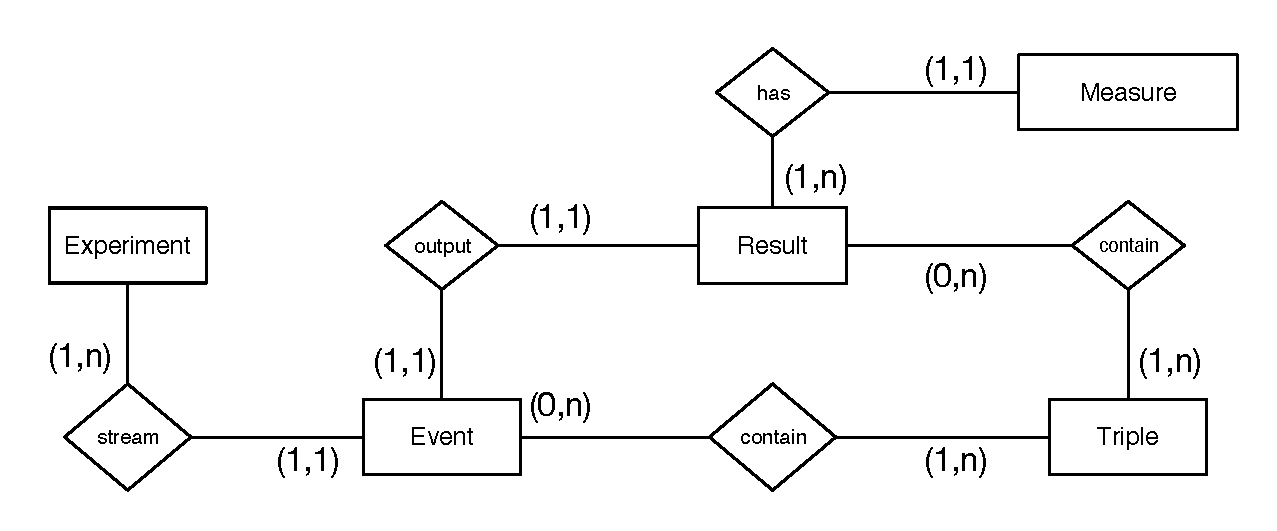
\includegraphics[width=\linewidth]{images/er-db}
	\caption{ER-Diagram For Experiment Output} 
  	\label{fig:er}
\end{figure}\\
\noindent\textsc{Experiment}(\underline{ID}, Timestamp Start, Timestamp End, Engine, Ontology, Query, Dataset, Description)\\
\textsc{Event}(\underline{ID, Experiment ID}, Timestamp)\\
\textsc{Result}(\underline{Result ID, Experiment ID}, Event ID)\\
\textsc{Measure}(\underline{ID}, Value)\\
\textsc{Measurement Set}(\underline{Measure ID, Result ID, Experiment ID})\\
\textsc{Triple}(\underline{S,P,O})\\
\textsc{Output Triple}(\underline{Result ID, Experiment ID, S, P, O})\\
\textsc{Input Triple}(\underline{Event ID, Experiment ID, S, P, O})\\

The \textsc{Experiment} entity contains all the metadata of the tuple $<\mathcal{E},\mathcal{D},\mathcal{T},\mathcal{Q},>$, which semantic is explained above. "Timestamp Start" and "Timestamp End" are relevant metrics for further analysis and system control. 
The \textsc{Event} is unique inside an \textsc{Experiment}, it is possible to send two events with the same timestamp and identical tripleset. The \textsc{Result}  is associated with one and only one \textsc{Event}. It contains the results to the engine queries w.r.t the active window and the set of the measure gathered during the execution. The \textsc{Measurement Set} table represent the relation between the \textsc{Result} and a number of measure that may variate  to fulfil requirement [R.7] (extendible measurement set). We include the concept of the \textsc{Triple} in order to model the content of \textsc{Event and Result}. \textsc{Input Triple} and \textsc{Output Triple} are the tables which represent the relation between \textsc{Triple} and respectively \textsc{Event} and \textsc{Result}
%a file, which contains a tuple with the sensor data and metadata for each event passed during the experiment execution; a set of TriG files that represents the window materialisation at each cycle, even in case of incremental reasoning. (It is also possible to save the non-materialised window, in order to verify the Completeness and Soundness of the reasoning procedure for the baselines).
%In practice the Test Stand outputs results in time series format and  the Analyser toolset has to handle this kind of information. 

\noindent The \textsc{Test Stand} orchestrates the communication between the upstanding models, forcing the \textsc{Streamer} to push events to the RSP Engine and the \textsc{Result Collector} to listen the output and collect the results.  To explain its workflow we split the process at the points when the modules exchange events. Indeed, each message represents a different logic step in the experiment execution cycle and we have distinguished six different ones.

In step (1) the \textsc{Test Stand} take the experiment and start the execution.  The \textsc{Test Stand} executes the experiment $<\mathcal{E},\mathcal{D},\mathcal{T},\mathcal{Q},>$ stressing $\mathcal{E}$ for a certain period of time looping through the steps from (2) to (5) illustrated in Figure \ref{fig:architecture}.                                                                                                                                                                                                                                                                                                                                                                                                                                                                                                                                                                                                                                                                                                                                                                                                                                                                                                                                                                                                                                                                                                                                                                                                                                                                                                                                                                                                                                                                                                                                                                                                                                                                                                                                                                                                                                                                                                                                                                                                                                                                                                                                                                                                                                                                                                                                                                                                                                                                                                                                                                                                                                                                                                                                                                                                                                                                                                                                                                                                                                                                                                                                                                                                                                                                                                                                                                                                                                                                                                                                                                                                                                                                                                                                                                                                                                                                                                                                                                                                                                                                                                                                                                                                                                                                                                                                                                                                      

In step (2), the \textsc{Streamer} pushes to $\mathcal{E}$ an event \textsc{CTEvent}. This event is a portion of an RDF Stream picked from the data $\mathcal{D}$ and it consists of a set of RDF triples with the same timestamp. In order to satisfy [R.12], it sends triple in N-Triple\footnote{\url{http://www.w3.org/2001/sw/RDFCore/ntriples/}}, which is the easiest RDF serialisation to parse.  

In step (3) $\mathcal{E}$ pushes to the \textsc{Result Collector} an event \textsc{OutCTEvent}. It contains the current answer to the query $\mathcal{Q}$ registered in $\mathcal{E}$ given the ontology $\mathcal{T}$. The \textsc{Test Stand} expects $\mathcal{E}$ to output result in N-Triple format. 

Notably, to place any RSP engine on the \textsc{Test Stand} (requirement [R.3]) \name provides a simple software wrapper that, when it receives a \textsc{CTEvent}, adapts it to the RSP engine specific format, pushes it in the RSP engine, and listens to the RSP engine output so to transform such an output in a \textsc{OutCTEvent}.

To measure performances (requirement [R.6]) the \textsc{Test Stand} performs several actions both before step (2) and after step (3) to collect data from the sensors. In step (4), those observations are added to the outputs of $\mathcal{E}$ as annotations and are pushed to the \textsc{Result Collector}.  We name \textsc{TSResult} the event that contains the sensor data plus the query results produced by the engine.  The \textsc{Test Stand} works in a single thread mode, blocking the execution of its components when it performs the measurements in (2) and (3) [R.4].  

Previous works about Stream reasoning \cite{} shows that the minimal performance measure set includes \textbf{Latency} -- defined as the delay between the injection of an event in the RSP engine and its response to it --, \textbf{Memory Load} -- defined as the difference between total system memory and the free one --, and \textbf{Completeness \& Soundness} of query-answering results. To measure latency, it starts a timer before (2) and stops it after (3). To measure memory load, it asks for the free memory of the system after step (3).

In step (5) the \textsc{Result Collector} saves \textsc{TSResult} for post process analysis [R.9], executed trough the \textsc{Analyzer}. It does so saving the content of any TSResult  [R.8].

\section{Baselines}
\label{sec:baselines}

\noindent In Chapter \ref{chap:problem-settings} we state that a Systematic Comparative Research Approach needs initial terms of comparison to lead the investigation. \name contains a set simple and easy-to-use RSP Engines called "baselines", developed to fulfil this lack . 
We exploit them to define some qualitative methods of investigation and to prove the usability of the Test Stand. 

In section \ref{sec:requirements} we identifies four characteristics that classify a case-study as a baseline inside a research field and here we report how \name Baselines are \textit{Elementary}, \textit{Relevant}, \textit{Simple} and \textit{Eligible}.

Early works on SR \cite{DBLP:conf/fis/ValleCBBC08,Walavalkar08streamingknowledge} describe the most simple approach to create a stream reasoning system: pipelining a DSMS with a reasoner. The DSMS is responsible to handle the data stream, moving from infinite sequences to finite (and processable) sets of events. The reasoner instead applies SPARQL queries on this set of events, exploiting its reasoning capabilities over a context that can be considered as static, but remains continuous.  As explained in Section \ref{sec:sfp}, we focus on this three the Stream Reasoning main building blocks: \begin{enumerate}
\item[1.] RDF streams;
\item[2.] An extensions of SPARQL to manage continuos data
\item[3.] reasoning algorithms
\end{enumerate}

\begin{figure}[tbh]
  \centering
	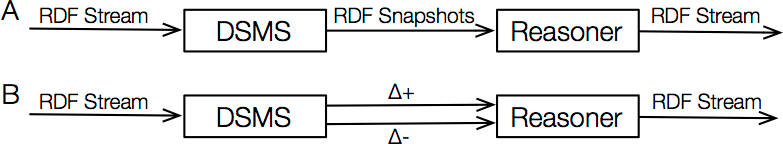
\includegraphics[width=\linewidth]{images/baselines-final}
	\caption{A: the architecture of the Naive baselines. B: the one of  the Incremental ones.} 
  	\label{fig:baselines}
\end{figure}
These there elements are summarised into RSP Engines, systems that can apply reasoning techniques upon rapidly changing information (Section \ref{sec:rspengine}). The approach above allow to develop an RSP Engine focusing only on link two existing technologies and develop the communication between them. But, how this design model fulfil the requirements poses in Section \ref{sec:requirements}?

Baselines \textit{Elementarity} is easy to be granted. The architecture above demands to choose a  DSMS which is a reliable solution in the CEP context  and the a general purpose rule engine which can be consider in the same way. We can consider this goal as reached when the couple elements are simple and valid terms of comparison w.r.t the state of the art.  Baselines \textit{Relevance} means to cover all the most important theoretical variants that the "pipeline approach" conveys. In terms of reasoning we can choose between to possible approaches and with reference to the data stream processing we have again two choice. Four baseline implementations cover these two main design decisions about the RDF Stream Model and the Reasoning procedures. 

The RDF Stream model describes how the input RDF Stream is processed, different systems accept data in different models, which depends on how RDF Stream is considered in terms of events contemporaneity. The two most relevant ones are:

\begin{itemize}	
\item Triple-based model, where the events pushed in the DSMS are timestamped triples. The timestamps are non decreasing, different triples could have the same timestamp to denote that they are contemporary.
\item RDF Graphs-based: the event pushed in the DSMS are timestamped RDF graph. The timestamps are increasing and the graph is used as a form of punctuation \cite{Tatbul2003b} to separate consequent portions of the RDF stream.
\end{itemize}

The Reasoning Architecture, the techniques to make inference, depends on the way data flow from the DSMS to the reasoner. Two reasoning solutions exist for the two triples data flow:

\begin{itemize}
\item Naive solution: (Figure \ref{fig:baselines}-A) the DSMS produces an RDF Snapshot of the current windows. Tt sends the entire content of the window to the reasoner, which materialises all the implied triples at each cycle. This is the approach implemented in the C-SPARQL Engine \cite{DBLP:journals/sigmod/BarbieriBCVG10} and in Sparkwave \cite{DBLP:conf/debs/KomazecCF12}.
\item Incremental solution (Figure \ref{fig:baselines}-B) the DSMS outputs the IRStream, the differences between the current window and the previous one. The $\Delta^{+}$ snapshot contains the triples that have just entered in the window, while the $\Delta^{-}$ snapshot contains the triples that have just exited from the window. The reasoner, using $\Delta^{+}$ and $\Delta^{-}$, incrementally maintains the materialisation over time. This approach is taken as term of comparison in \cite{DellAglio2014} and it is inspired from \cite{DBLP:conf/cikm/RenP11}.
\end{itemize}

Baseline \textsc{Eligibility} requires to check out all the performance measurements involved by the RSP Engine in use. We already stated that the choice of the DSMS and the reasoned may affect baseline \textsc{Elementarily}, but they also influence the performance of the engine. As reported in Section \ref{sec:teststand}, we take as initial measure set: Latency, Memory and of the query results Completeness and Soundness. The baselines must be at least comparable with commercial solutions in terms of degree of magnitude, in order to be Eligible for Latency and Memory. More consideration on this metrics are presented in Chapter of \ref{chap:evaluation}, which deeply answers the question with experimental results. On correctness of RDF stream processing \cite{DBLP:conf/semweb/DellAglioCBCV13} previous works explain the importance of external control on time to assure that the RSP Engine always outputs the correct answers (even when overloaded). The proposed baselines should take advantage of the ability of some DSMS to be temporally controlled by an external agent by sending time-keeping events to synchronise the internal time flow. %One time-keeping event is sent before injecting the triples in a \textsc{TCEvent} and another one after all triples in \textsc{TCEvent}  were sent. In this way all the triples in the TCEvent are consider contemporary by the 

Finally, baselines \textsc{Simplicity} comes from those parameters that directly influence the RSP Engine: the query $\mathcal{Q},$ and the entailment regime. $\mathcal{Q}$ should be eligible in terms of reasoning which means having an high materialisation effort of the implicit information entailed by the content of the window, given the ontology chosen by the user. The entailment regime should be a fragment of a language, maybe RDF-S,  which reduce complexity but preserves the normative semantics and the core functionalities. Moreover, what we state above about externally time control clarify the system workflow, so it is demanded to sustain baselines \textsc{Simplicity} too.

\section{Analyser}\label{sec:analyser}

The Analyser is conceptually a set of tools that allows visualisation and statistical investigation of the result data . As reported in Section \ref{sec:teststand}, the Test Stand executes \textsc{experiments} and produces times series, whose study is a very wide matter. To this extent, it is hard to think the Analyser in a general way. Another motivation regards the relation between the hypothesis and    tools to apply the analysis. The first one depends on the the research question, while the second one requires to study the data, which are related to the experiment. 

However, it is possible to identify some common characteristics that have a general meaning. Independently from the hypothesis and  experiment we can consider many investigation methods, in particular the Systematic Comparative Approach presented in Chapter \ref{chap:problem-settings}), which demands to identify characteristics upon which is possible to build comparison. 

\begin{figure}[tbh]
  \centering
	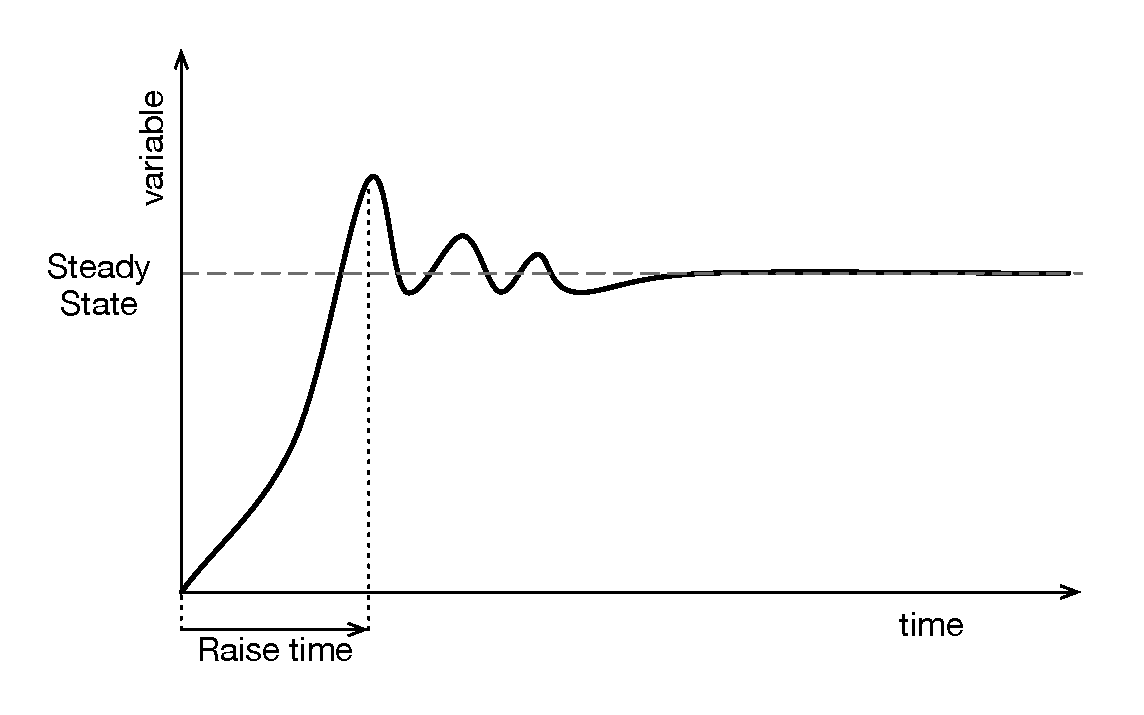
\includegraphics[width=0.5\linewidth]{images/steady-state}
	\caption{Time Series temporal domain} 	
  	\label{fig:steady-state}
\end{figure}

First of all, the Analyser tool-set must include an automatic procedure average the data of multiple execution of the same experiment. Even if the Test Stand is designed to be system independent, it is a dynamic system as the ones we want to study. Strange results may happen while an experiment is running. In order to reduce and possible eliminate the outliers, multiple runs of the same experiment must be mediated obtaining the average measures. 

Once we have reliable data, we can decline the comparative research approach either to the visual analysis or statistical investigation. The first method is more qualitative then the second one, but read the information presented in graphical way can be preferred in the primary steps of a study. On the other hand, the statistical investigation method demands more complex instruments to interpret the data, but allows to answer also elaborate questions.

Time series studies usually start with data visualisation analysis. The most common plotting tools represent the series in temporal form. Moreover, it is relevant to visualise their behaviour in the frequency domain. 

The Steady State is the moment when a dynamic system reaches the equilibrium for a certain variable. The identification of this condition is a common passage in almost any research on dynamic system and visual analysis can be exploited as the simplest tool to complete the task. Figure \ref{fig:steady-state} shows a typical behaviour for a system in the time domain and also evidences the point when the the serie reaches the Steady State condition. Visualise the point of when Steady State is reached is useful to exclude the initial warm-up period form the data and properly verify hypothesis. Anyhow, this method is limited, it must be applied for each system variable, because they may reach the equilibrium at different times.

\begin{figure}[tbh]
  \centering
	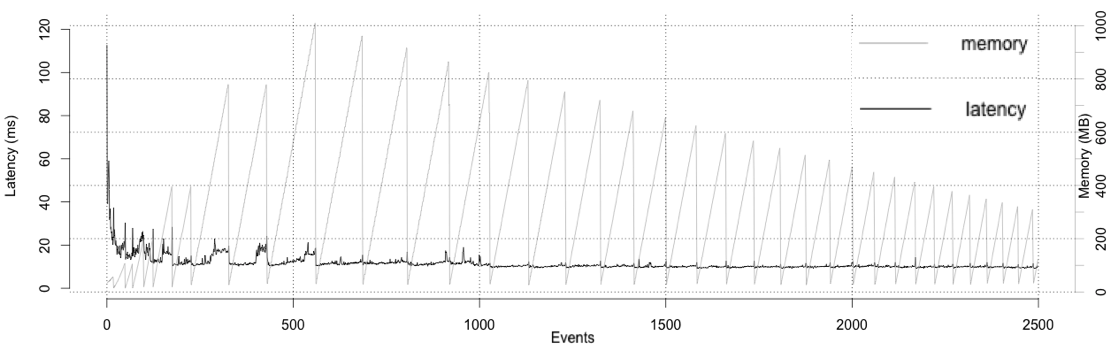
\includegraphics[width=0.80\linewidth]{images/comp-intra}
	\caption{Intra Experiment Comparison} 
  	\label{fig:comp-intra}
\end{figure}

Independently from the Steady State condition, variables relation can be evidenced in a comparative form and the Analyser must support this kind of studies. We distinguish three main investigation options, the following images show a some examples of them:
% A) Intra-Experiment Comparison ; B) Inter-Experiment Comparison; C) Pattern Recognition. T

\begin{figure}[tbh]
  \centering
	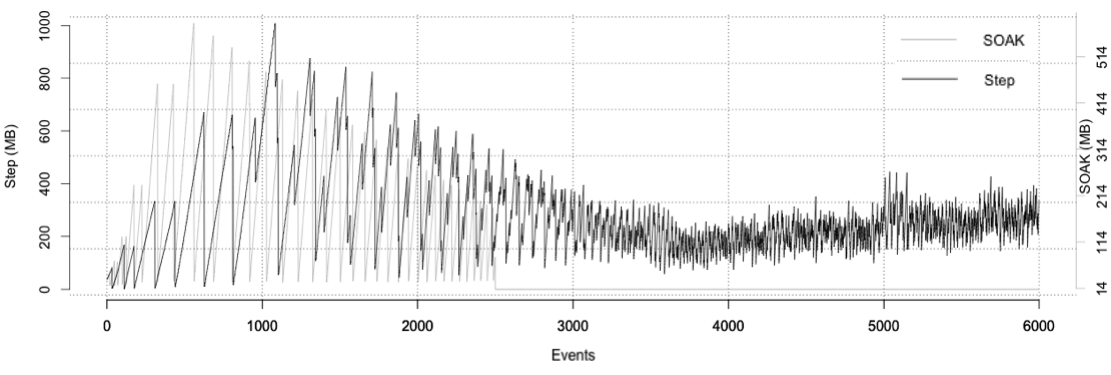
\includegraphics[width=0.80\linewidth]{images/comp-inter}
	\caption{Inter Experiment Comparison} 
  	\label{fig:comp-inter}
\end{figure}

\begin{enumerate}
\item[A] Figure \ref{fig:comp-intra} shows an example of intra-experiment investigation, multi-plotting them on the time domain or frequency domain; 
\item[B] Figure \ref{fig:comp-inter} shows an example of inter-experiment investigation: multi-plotting the same variable, arguing about the similarity or the difference upon a certain fixed characteristic.  
\item[C] Figure \ref{fig:patterns}  shows an example of pattern recognition: inter-experiment on the same variable or intra-experiment on the relation between variable;
\end{enumerate}

\begin{figure}[tbh]
  \centering
	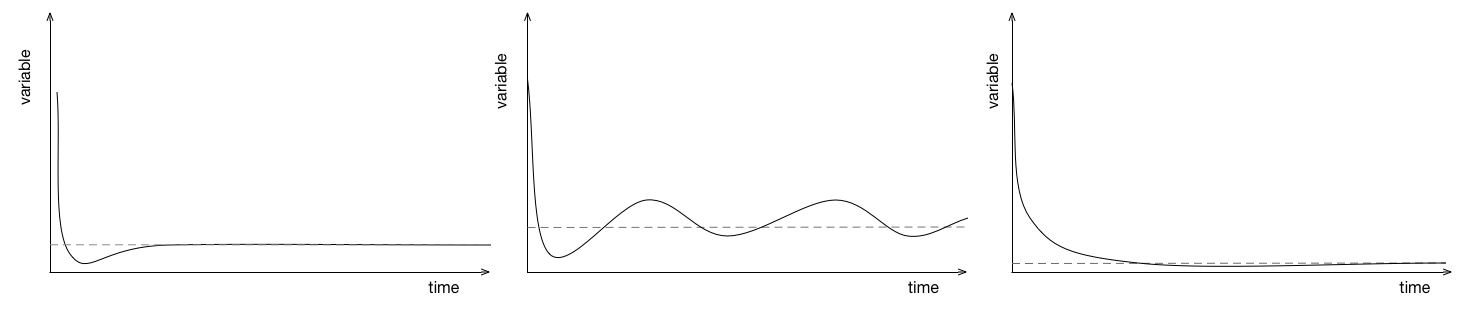
\includegraphics[width=0.85\linewidth]{images/patterns}
	\caption{Pattern recognition example} 
  	\label{fig:patterns}
\end{figure}

\pagebreak

The Analyser has to supports also hypothesis on system behaviour changes: a time serie describes how a dynamic system evolves over time, so it is meaningful to attempt hypothesis verification trough statistical operations,which always consider the the Steady State to obtain general answers to our questions. The most common metrics are average and standard deviation and maximum or minimum for a certain variable. Upon this calculated data is possible to compare experiments or variable in a global manner, drawing a solution space. 
The options of intra-experiment and inter-experiment comparisons are still meaningful, and now we can chose to look at numeric values or to provide only an analysis of the system trend. Pattern identification is quite harder than in the visual analysis approach, because it depends on the data representation. Tables \ref{tab:comp-tables} (a) and (b) show two example of statistical analysis with different detail levels. How to choose the proper level depends on the needs of the research:

\begin{table}[htb]
\scriptsize
	\centering
	\subtable[Symbolic Comparison of variables A vs B on Experiment 1]{%
		\begin{tabular}{c | cccc} % creating eight columns
	  	\hline
		A vs B & \multicolumn{4}{c}{Experiment 1 Condition A}  \\
		 Comparison  & &&&\\
		\hline
		   	        & $\simeq$\\
		 Experiment 1 & A     & 	$\simeq$  & A & B\\
		 Condition  & A     & 	$\simeq$  & $\simeq$ & B\\
		 B          & A     & 	$\simeq$  & B & A\\
		\hline % inserts single-line
	 \end{tabular}
	}\qquad\qquad
	\subtable[Symbolic Comparison of variables A vs B on Experiment 1]{%
		\begin{tabular}{c | cccc} % creating eight columns
	  	\hline
		A vs B & \multicolumn{4}{c}{Experiment 1 Condition A}  \\
		 Comparison  & &&&\\
		\hline
		   	        & $\simeq$\\
		 Experiment 1 & 10\%     & 	$\simeq$  & 42\% & 33\%\\
		 Condition  & 23\%     & 	$\simeq$  & $\simeq$ & 12\%\\
		 B          & 20\%    & 	$\simeq$  & 22\% & 22\%\\
		\hline % inserts single-line
	 \end{tabular}
	}
	\caption{(a) intra experiment-comparison over two variables - (b) inter-experiment comparison over a common variable }
	\label{tab:comp-tables}
\end{table}

Last but not least, since data mining procedures are very system-dependent we decide to include examples of possible analysis in Chapter \ref{chap:evaluation} about the experimental evaluation of the Baselines. The purpose of Chapter \ref{chap:evaluation} is both to demonstrate the value of \name and to provide some guidelines for further evaluations.




